\chapter[Introduction]{Introduction} \label{cha:introduction}
This section of the report will explain to the reader how to reference this document and explain the fundamental structure of the project as well as the report.
\section{Reading comprehension}
Throughout the report, the reader will be assumed to be knowledgeable of basic circuit analysis and familiar with standard abbreviations typically used in electrical engineering. If not, readers can refer to the denotation section at the beginning of the report.

Please refer to \hyperref[cha:abbr]{Abbreviation page} and \hyperref[cha:denotation]{Denotation page} for abbreviations and variable names found within the report.

Furthermore, as a notation convention, large-signal DC quantities are denoted by uppercase letters with uppercase subscripts. Small-signal quantities are denoted using lowercase letters with lowercase subscripts. Quantities composed of both large-signal and small-signal elements are denoted using lowercase letters and uppercase subscripts.

\subsection{Sources}
Calculus expressions present in the report will typically have a reference explaining their origin. All references are prominently displayed with square brackets and a number, directing to the appendix in the last section of the report.

\subsection{Report structure}
The report is divided into five chapters, where the first part is an introduction to the project. The second chapter will focus on explaining the theory of a class-D amplifier with its modulation schemes and output filter. The third chapter focuses on the synthesis of a PCB to test. The fourth chapter explains the production of the hardware. The fifth chapter will explain the testing methodology performed on the hardware. Finally, the documentation of testing and diagrams of laboratory setups can be found in the appendix.

\section{Project description} \label{sec:1.2_project_description}
In the following report, an analysis of a class-D amplifier module is documented. The work is conducted in the Department of Electrical Engineering at the \organisation. \\\\
An audio amplifier is a device that amplifies low-power audio signals within the audio spectrum perceptible to the human hearing to a level suitable for loudspeakers. It is typically the second last stage in an audio playback chain. While the input signal to an audio amplifier measures a low power, the output of the amplifier typically measures a high power delivery to the load, in this case, a loudspeaker. The output power of the amplifier depends on several key factors, characteristics of the output stage, heat dissipation, and parasitic elements among others. \\\\
A class-D audio amplifier is a typology of audio amplifiers that utilizes transistors as switches instead of gain devices as in other amplifier systems. As the transistors are operating non-linearly, the input signal is converted into a stream of pulses that resemble the input signal through a pulse-width modulation scheme. The time-averaged power of the modulated pulses is directly proportional to the input signal, so after amplification, the signal can be converted back into an analog signal through a passive low-pass filter. The purpose of this filter is to reduce high-frequency components in the amplified signal and thereby restore the audible spectrum frequency signal. \\

\begin{figure}[htbp]
    \centering
    

\tikzset{every picture/.style={line width=0.75pt}} %set default line width to 0.75pt        

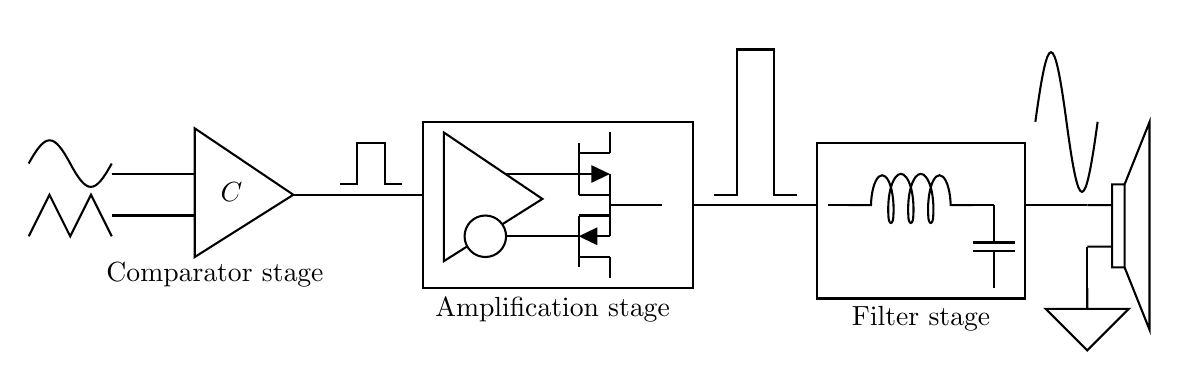
\begin{tikzpicture}[x=0.75pt,y=0.75pt,yscale=-1,xscale=1]
%uncomment if require: \path (0,170); %set diagram left start at 0, and has height of 170

%Shape: Rectangle [id:dp770054193310846] 
\draw   (195,40) -- (325,40) -- (325,120) -- (195,120) -- cycle ;
%Shape: Sine Wave Form [id:dp7770371160645917] 
\draw   (5,59.95) .. controls (13.14,45.08) and (16.98,45) .. (25,59.95) .. controls (33.02,74.91) and (36.79,75) .. (45,59.95) ;
%Shape: Triangle [id:dp07335766351707096] 
\draw   (132.5,75) -- (85,105) -- (85,43) -- cycle ;
%Straight Lines [id:da9002322344892075] 
\draw    (45,65) -- (85,65) ;
%Straight Lines [id:da9755027100331979] 
\draw    (45,85) -- (85,85) ;
%Shape: Boxed Line [id:dp8415560598999601] 
\draw    (45,95) -- (35,75) -- (25,95) -- (15,75) -- (5,95) ;
%Shape: Pulse Wave Form [id:dp983169087343869] 
\draw   (155,70) -- (163.33,70) -- (163.33,50) -- (176.67,50) -- (176.67,70) -- (185,70) ;
%Straight Lines [id:da26299434651745646] 
\draw    (132.5,75) -- (195,75) ;
%Shape: Triangle [id:dp7248202440259415] 
\draw   (252.5,77) -- (205,107) -- (205,45) -- cycle ;
%Straight Lines [id:da4440606939859202] 
\draw    (235,65) -- (270,65) ;
%Shape: Circle [id:dp46389042827957394] 
\draw  [fill={rgb, 255:red, 255; green, 255; blue, 255 }  ,fill opacity=1 ] (215,95) .. controls (215,89.48) and (219.48,85) .. (225,85) .. controls (230.52,85) and (235,89.48) .. (235,95) .. controls (235,100.52) and (230.52,105) .. (225,105) .. controls (219.48,105) and (215,100.52) .. (215,95) -- cycle ;
%Straight Lines [id:da7398031594417624] 
\draw    (235,95) -- (270,95) ;
%Shape: Pulse Wave Form [id:dp1410329557987886] 
\draw   (335,75) -- (346.11,75) -- (346.11,5) -- (363.89,5) -- (363.89,75) -- (375,75) ;
%Straight Lines [id:da796082230836703] 
\draw    (325,80) -- (385,80) ;
%Shape: Rectangle [id:dp4920940793193982] 
\draw   (385,50) -- (485,50) -- (485,125) -- (385,125) -- cycle ;
%Straight Lines [id:da5196077455553685] 
\draw    (390,80) -- (400,80) ;
%Shape: Inductor (Air Core) [id:dp38851992124783474] 
\draw   (400,80) -- (410.8,80) .. controls (410.96,73.64) and (412.45,68.2) .. (414.58,66.3) .. controls (416.7,64.4) and (419.01,66.42) .. (420.4,71.39) .. controls (421.47,75.28) and (421.91,80.29) .. (421.6,85.16) .. controls (421.6,87.06) and (421.06,88.61) .. (420.4,88.61) .. controls (419.74,88.61) and (419.2,87.06) .. (419.2,85.16) .. controls (418.89,80.29) and (419.33,75.28) .. (420.4,71.39) .. controls (421.65,67.26) and (423.38,64.92) .. (425.2,64.92) .. controls (427.02,64.92) and (428.75,67.26) .. (430,71.39) .. controls (431.07,75.28) and (431.51,80.29) .. (431.2,85.16) .. controls (431.2,87.06) and (430.66,88.61) .. (430,88.61) .. controls (429.34,88.61) and (428.8,87.06) .. (428.8,85.16) .. controls (428.49,80.29) and (428.93,75.28) .. (430,71.39) .. controls (431.25,67.26) and (432.98,64.92) .. (434.8,64.92) .. controls (436.62,64.92) and (438.35,67.26) .. (439.6,71.39) .. controls (440.67,75.28) and (441.11,80.29) .. (440.8,85.16) .. controls (440.8,87.06) and (440.26,88.61) .. (439.6,88.61) .. controls (438.94,88.61) and (438.4,87.06) .. (438.4,85.16) .. controls (438.09,80.29) and (438.53,75.28) .. (439.6,71.39) .. controls (440.99,66.42) and (443.3,64.4) .. (445.42,66.3) .. controls (447.55,68.2) and (449.04,73.64) .. (449.2,80) -- (460,80) ;
%Shape: Capacitor [id:dp0005959816196527967] 
\draw   (470,80) -- (470,98) (480,102) -- (460,102) (480,98) -- (460,98) (470,102) -- (470,120) ;
%Straight Lines [id:da7273075387286561] 
\draw    (460,80) -- (470,80) ;
%Shape: Sine Wave Form [id:dp8404377662111795] 
\draw   (490,39.86) .. controls (496.1,-4.77) and (498.98,-5) .. (505,39.86) .. controls (511.02,84.72) and (513.84,85) .. (520,39.86) ;
%Shape: Speaker [id:dp7858617504965892] 
\draw   (545,140) -- (545,40) -- (533,70) -- (527,70) -- (527,110) -- (533,110) -- (545,140) -- cycle (515,100) -- (527,100) (515,80) -- (527,80) (533,70) -- (533,110) ;
%Shape: Ground [id:dp5397046528572682] 
\draw   (495,130) -- (515,150) -- (535,130) -- (495,130) -- cycle (515,120) -- (515,130) ;
%Straight Lines [id:da4445340304920644] 
\draw    (515,100) -- (515,120) ;
%Straight Lines [id:da295419950659239] 
\draw    (515,80) -- (485,80) ;
%Straight Lines [id:da820180143723801] 
\draw    (270,50) -- (270,75) ;
%Straight Lines [id:da7237066207339522] 
\draw    (270,65) -- (282,65) ;
\draw [shift={(285,65)}, rotate = 180] [fill={rgb, 255:red, 0; green, 0; blue, 0 }  ][line width=0.08]  [draw opacity=0] (8.93,-4.29) -- (0,0) -- (8.93,4.29) -- cycle    ;
%Straight Lines [id:da9331978539015273] 
\draw    (270,55) -- (285,55) ;
%Straight Lines [id:da935543339026137] 
\draw    (285,55) -- (285,45) ;
%Straight Lines [id:da22661795044798372] 
\draw    (270,75) -- (285,75) ;
%Straight Lines [id:da4597083380977842] 
\draw    (285,65) -- (285,80) ;
%Straight Lines [id:da6624762220456999] 
\draw    (285,80) -- (310,80) ;
%Straight Lines [id:da7506799387821979] 
\draw    (285,75) -- (285,85) ;
%Straight Lines [id:da910108528126899] 
\draw    (270,85) -- (285,85) ;
%Straight Lines [id:da49163459588421765] 
\draw    (270,85) -- (270,110) ;
%Straight Lines [id:da5333620114017099] 
\draw    (285,95) -- (273,95) ;
\draw [shift={(270,95)}, rotate = 360] [fill={rgb, 255:red, 0; green, 0; blue, 0 }  ][line width=0.08]  [draw opacity=0] (8.93,-4.29) -- (0,0) -- (8.93,4.29) -- cycle    ;
%Straight Lines [id:da3270452113061644] 
\draw    (285,85) -- (285,95) ;
%Straight Lines [id:da5095926548035659] 
\draw    (270,105) -- (285,105) ;
%Straight Lines [id:da3825574463791581] 
\draw    (285,115) -- (285,105) ;

% Text Node
\draw (96,67.4) node [anchor=north west][inner sep=0.75pt]    {$C$};
% Text Node
\draw (37,106) node [anchor=north west][inner sep=0.75pt]   [align=left] {\begin{minipage}[lt]{84.36216pt}\setlength\topsep{0pt}
\begin{center}
Comparator stage
\end{center}

\end{minipage}};
% Text Node
\draw (197,123) node [anchor=north west][inner sep=0.75pt]   [align=left] {\begin{minipage}[lt]{88.33608000000001pt}\setlength\topsep{0pt}
\begin{center}
Amplification stage
\end{center}

\end{minipage}};
% Text Node
\draw (398,127) node [anchor=north west][inner sep=0.75pt]   [align=left] {\begin{minipage}[lt]{53.17810800000001pt}\setlength\topsep{0pt}
\begin{center}
Filter stage
\end{center}

\end{minipage}};


\end{tikzpicture}

    \caption{Block diagram of basic class-D amplifier topology.}
    \label{fig:01_classd_diagram}
\end{figure}

See \autoref{fig:01_classd_diagram} for a block diagram overview of a class-D amplifier system with waveform illustrations.
The primary benefit of the class-D topology is an increased power efficiency as the maximum theoretical power efficiency for class-D amplifiers are near 100\%, whereas Class-A- and Class-B amplifiers maximum theoretical power efficiency is 25\% and 78.5\%, respectively.\\

The design process in this project will be based on previous work by \cite{multivar_ctrl_loops_for_SM_audio_systems,nagy_special_course}. These two works explored using LQR in a control loop and minimizing the generated noise within the circuit from that implementation. The result was a circuit design that was implemented in-house within the DTU laboratory that is documented through an iterative design process.

\section{Project scope}
As this project deals with a synthesis of a peculiar design and an analytical examination of a class-D system, this initial design will determine the specific direction of the qualitative analysis. The project is focused on the output stage of the system. Therefore analysis will comprise of distinctive variations of parasitic element combinations in the chosen output filter topology.

\subsection{Learning objectives}
See below for an outline of the project activities
\begin{table}[htbp]
    \centering
    \begin{tabular}{@{}l@{}}
    	\toprule
        \textbf{Project specification}									\\ \midrule
        Learn a class-D amplifier topology, calculate component values	\\
        Understand and design a self-oscillating modulator amplifier	\\
        Investigate and test open loop output filter					\\
        Investigate and test closed loop output filter					\\
        Investigate output filter parasitic elements affects control loop\\
        Make quantifiable performance measurements on system			\\
        Write a technical report documenting the project work			\\ \bottomrule
    \end{tabular}
    \caption{Project specification table}
    \label{tab:specifications}
\end{table}